\documentclass{article}
\usepackage{graphicx}
\graphicspath{{images/}}
\begin{document}
	\title{COMP3204\\Computer Vision\\Lecture Notes}
	\author{Bradley Mason}
	\maketitle
	
	\newpage
	\tableofcontents
	\newpage
	
	\section{Vision Models}
	\subsection{Physical Model}
	The physical model is the eye. It is involved from defence/survival. You form the image on the \textbf{fovea} and shape your lens. There are many image sensors, of type \textbf{rod} and \textbf{cone}.\\
	\\\textbf{Rods }help you to see black and white images (monochrome), this is called \textbf{scotopic vision}.\footnote{vision of the eye under low light conditions}\\
	There are in the order $10^8$ rods and they all lie just off the fovea.\\
	\\\textbf{Cones} help you to see colour images, this is called \textbf{photopic vision}.\footnote{vision of the eye under well lit conditions}\\
	There are in the order $10^7$ cones which lie on the fovea but most are just on the edge. They can interpret three types of wavelength:
	\begin{itemize}
		\item Short = Blue (UV)
		\item Medium = Green/Yellow
		\item Long = Red (IR)
	\end{itemize}
	The eye is bad at seeing blue so it compensates by letting in more blue light. Also there isn't enough bandwidth in the eye to handle all the sensor data, this suggests that there is some form of coding.\\
	On a side note you eye is also subject to \textbf{mach bands}. This is where differing shades of grey meet in an image causing the eye to see an exaggerated contrast and a line on the edge. It is the brain's method of edge detection that causes you to see elements that don't exist.
	\subsection{Neural Model}
	This was found by experiments, the neural model is within the brain where signals are combined and mathematical models are applied. This can be justified with experiments.\\
	There is a new find of LGN, the Lateral Genicular Nucleus.
	\subsection{Processing/Psychology}
	Actions happen in both the \textbf{occipital} cortex and the \textbf{associative} cortex. Within the occipital you perceive texture but this requires training and is easily deceived.\\
	The associative cortex finds links.
	
	\section{Fourier}
	Images are stored as 8-bit bytes. There are about 6dB per bit, for comparison video has a bandwidth of roughly 48dB. However human vision is around 5 bits.
	\subsection{Resolution}
	Resolution is stored in $2^n*2^n$ for efficiency. You should always use the smallest resolution suitable for the task but how do you determine what is a suitable resolution?
	\subsection{Fourier Transform}
	The Fourier transform guides resolution, it provides us with a new way to understand the image.\\
	Spacial Image $\Longleftrightarrow$ Frequency\\
	You go forward with the Fourier Transform and backwards with the inverse. For example think of a music graphics equaliser frequency levels.\\
	$\omega=$frequency and t=time in:
	$$F(\omega)=\int_{-\infty}^{\infty}f(t)e^{-j\omega t}\delta t$$
	$$=\int_{\frac{-T}{2}}^{\frac{T}{2}}Ae^{-j\omega t}\delta t$$
	$$=A\frac{e^{-j\omega t}}{-j\omega}\mid_{-T/2}^{T/2}$$
	$$=A(\frac{e^{-j\omega\frac{T}{2}}-e^{-j\omega\frac{T}{2}}}{-j\omega})$$
	$$=\frac{2A}{\omega}\sin(\frac{\omega T}{2})$$
	Fourier has both magnitude (how much) and phase (when).
	\subsection{Sampling}
	Very fast sampling = high resolution.\\
	Very slow sampling = low resolution.\\
	Nyquist Theorem = "\textit{Sample at twice the maximum frequency}". Video is 2D so there is no theorem but the general guideline is 2 points per feature of interest.
	\subsection{Discrete Fourier Transform}
	$$F(U_i)=\sum_{i}U_ie^{-j(it)}$$
	Where $U_i$ is the discrete set of points.\\
	This is implemented by the fast fourier transform. Sampled points + sampled frequencies.
	\subsection{Applications}
	This can be applied to textures to understand the image, coding via frequency content, representation or even just to speed up algorithms.
	\section{Point Operators}
	This is where images are described by the histogram. We can use a point operators map, the new point is some function on the old point. $N_{x,y}=f(O_{x,y})$\\
	We need this to be automatic, for instance intensity normalisation. This smooths out the curve of what the pixels consist of to be equal across the spectrum. The range is the original max minus min. The scale is then 255 divided by the range. The new point (normalised) is the scale multiplied by the subtraction of the original min from the current point. This gives a linear stretch occupying all grey levels.
	\subsection{Histogram Equalisation}
	TO equalise you flatten the histogram. This is aimed at being better for human vision, you aim for a flat histogram. This is non-linear and meant for an NxN image. The number of old points equals the new, the number of points in the new up to a brightness level is the same as the old up to some other brightness level.
	$$\sum_{l=0}^{q}N(l)=\sum_{l=0}^{p}O(l)$$
	From this you can deduce that $q=\frac{255}{N^2}\sum_{l=0}^{P}O(l)$.\\
	This gives a mapping function into equalised images. Equalisation is absolute, repeating it will have no effect. This is used for display \textbf{ONLY} because it is non-linear.
	\subsection{Thresholding}
	$N_{x,y}=\mid_0^1$\\
	$O_{x,y}\geq$ threshold, otherwise\\
	The bar represents a conditional operation.\\
	There are many variants such as Otsu's "optimal" thresholding.
	\section{Group Operators}
	You form the image by combining points in regions, this is implemented by \textbf{template convolution}.
	$$N_{x,y}=\sum_{i\in region}\omega_i*O_i$$
	There are multiple ways to deal with the edges/borders. Setting them to black is the easiest, a complex method is to use a smaller region at the borders or, you can use Fourier assumption to allow them to wrap-around.
	\subsection{Averaging}
	$\omega_i=1/$window size area
	\subsection{Gaussian Averaging}
	This is better averaging at a time cost, you calculate $\omega_i$ from the gaussian distribution - $e^{\frac{-(x^2+y^2)}{2\sigma^2}}$. $\omega_i$ depends on the window size and $\sigma$(s.d).\\
	A large sigma gives similar to direct average whereas a small sigma gives no averaging.\\
	This method is great for gaussian distribution due to the noise.
	\subsection{Median Averaging}
	This method maintains edges and removes noise better than other averaging methods.\\
	It lists the pixel values in the region then sorts and takes the median. This removes extreme white and black pixels\footnote{known as salt and pepper noise} and is also \textbf{optimal}.
	\subsection{Mode Operator}
	This method is great for \textbf{rally noise}\footnote{NO IDEA WHAT THIS IS} which is often found in medical imaging. However, this method requires more code and more time.
	\section{Edge Detection}
	This is done by detecting image contrast\footnote{Difference in intensity} using first order differentiation. Vertically adjacent points are analysed to find horizontal edges and horizontally adjacent points are analysed to find vertical edges. 
	\section{Finding Shapes}
	\textbf{Occlusion} is just organised noise, it blocks out part of the image. When finding shapes we group together edge points but simple thresholding is too simple, we need the shape.
	\subsection{Template Matching}
	\textbf{Template matching} is the best procedure:
	\begin{itemize}
		\item Take image and the template
		\item Accumulate matching points in the template for each point in the image (like convolution)
		\item The darkest point, the most accumulated, is the best point.
		\item This is optimised for noise and occlusion but is slow
		\item It can, however, be sped up with Fourier
		\item Template Matching = inverseFourier(Fourier(template) X Fourier(image)
	\end{itemize}
	\subsection{Hough Transform for lines}
	If you take y=mx+c where x,y are the points, m is the gradient and c is the intercept.\\
	You can then re-arrange to use m and c as the points to get multiple lines from points on the original line which all intercept at a point that represented the original line.\\
	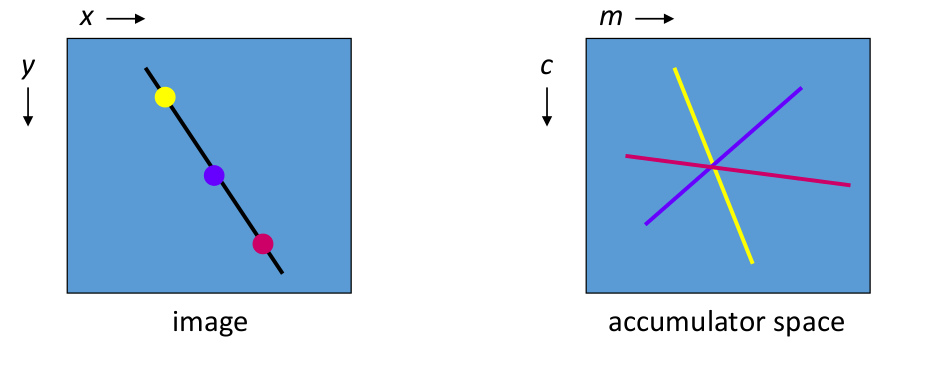
\includegraphics[scale=0.39]{houghtransform}
	\\
	argmax(accumulator) will give the peak. The pseudo code is as follows:
	\begin{verbatim}
	procedure:
	    for all x,y:                        !search image
	        {if image(x,t) >/ threshold     !find point
	            {for all m in Mmin,Mmax     !all values of n
	                {c=-xm+y
	                accumulator(m,c)+1}}}   !vote
	\end{verbatim}
	Afterwards, argmax(accumulator) gives values of the best m,c.\\
	This gives the same result as template matching but it's faster, it is also impractical due to Mmax being $\infty$ which causes an infinite loop.\\
	By using the polar equation though, we can avoid this issue.$$s\cos\theta + y\sin\theta = \rho$$
	This can be proved from the foot of the normal. You take $\theta$ between -90 and 90 and $\rho$ between 0 and N root 2 where N is the picture size.
	$$-90<\theta<90, 0<\rho<\sqrt{2}*N$$
	This means that all parameters are now constrained unlike the Cartesian equation.
	\subsection{Hough Transform for Circles}
	$$(x-x_0)^2+(y-y_0)^2=r^2$$
	For this equation we have two options for the points and centres of the circle. You can use x,y or $x_0$,$y_0$ for either. You have a radius r. It works very similar to lines except the equation produces circles.
	\begin{verbatim}
	for all x,y in image
	    {if edge(x,y) >/ threshold
	        {for all r in Rmin,Rmax
	            {for all theta in 1,360
	                {x0 = x+rcos()theta)
	                y0 = y+rsin(theta)
	                accumlator(x0,y0,r) += 1}}}}
	\end{verbatim}
	Afterwards search for the peak/maximum in accumulator.
	\subsection{Hough Transform for Ellipses}
	$$\frac{(x-x_0)^2}{a^2}+\frac{(y-y_0)^2}{b^2}=1$$
	This is a 4D accumulator, $x_0,y_0,a,b$ and if you add rotation it would become 5 dimensions.\\
	This means that for 100 value parameters and a 5D accumulator it has $10^{10}$ values. This gets very slow so requires special implementations.
	\subsection{Hough Transform for Arbitrary Shapes}
	To use the generalised Hough Transform you follow these steps:
	\begin{enumerate}
		\item Form a template
		\item Use template for voting
		\item Find peak
	\end{enumerate}
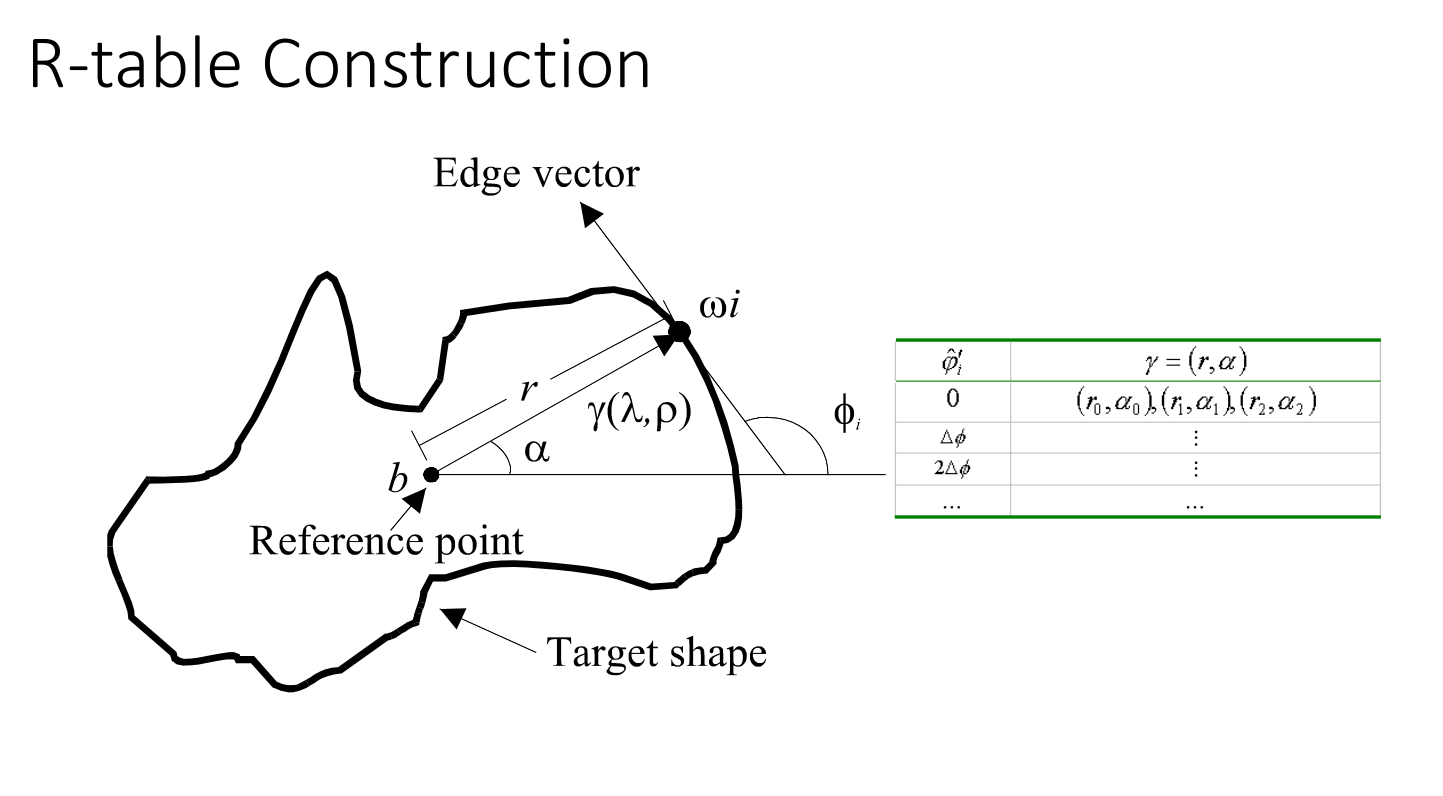
\includegraphics[scale=0.248]{rtableconstruct}
	The template is stored in an R-table, this contains distances and angle to the centre point. You then use $\phi$, the edge direction, as the index. Points with the same edge direction will be stacked to the right in the table and this is the noise. However, once you have attempted to apply an element of the table that has more than one entry, you must apply it uniformly which means the noise is uniform and thus easy to detect as noise.\\
	For rotation you add an offset to $\alpha$ or $\theta$, for scaling you multiply by r.
	
	\section{Building Machines That See}
	A CCD is better than CMOS for sensitivity and noise. Hence they are used in industrial applications of Computer Vision.\\
	Key terms in designing Computer Vision Systems:
	\begin{itemize}
		\item robust = what you want
		\item repeatable = what you want
		\item invariant = what you design your system to be
		\item constraints = what you apply to make it work
	\end{itemize}
	\subsection{Robustness}
	The vision system must be robustness to changes in its environment. For example, changes in lighting, angle or position of the camera etc...
	\subsection{Repeatability}
	Repeatability is the measure of robustness. It means that the system must work the same over and over, regardless of environmental changes.
	\subsection{Invariance}
	Invariance to environmental factors helps achieve robustness and repeatability. Hardware and software can be designed to be invariant to certain environmental changes e.g. you could design an algorithm to be invariant to illumination changes.
	\subsection{Constraints}
	Constraints are what you apply to the hardware, software and wetware to make your computer vision system work in a repeatable, robust fashion. E.g. you constrain the system by putting it in a box so there can't be any illumination changes.\\
	In industrial applications there are a lot more constraints on the environment which makes it easier to use and design for.
	\subsection{Software Constraints}
	Really simple but incredibly fast algorithms. The Hough transform is popular but note that it isn't all that robust without physical constraints. The same is true for most algorithms/techniques in industrial vision.\\
	The intelligent use of colour?
	\subsection{Colour Spaces}
	There are many different ways of numerically representing colour, a single representation of all possible colours is called a \textbf{colour-space}.\\
	It is generally possible to convert from one colour-space to another by applying a mapping in the form of a set of equations or an algorithm.\\
	Most physical image sensors capture \textbf{RGB}, this is by far the most widely known space. RGB couples brightness\footnote{\textbf{luminance}} with each channel, meaning that illumination invariance is very difficult.\\
	\textbf{HSV Colour-space} uses Hue, Saturation and Value as a colour-space. Hue encodes the pure colour as an angle, where red is at $0^o$. Remember that $0^o=360^o$!\\
	Saturation is how vibrant the colour is and the Value encodes the brightness. Using just H or H and S is a great way to achieve invariance to lighting.
	\subsection{Physical Constraints}
	Industrial vision is usually solved by applying simple computer vision algorithms, and lots og physical constraints:
	\begin{itemize}
		\item \textbf{Environment}: lighting, enclosure, mounting
		\item \textbf{Acquisition Hardware}: expensive camera, optics, filters
	\end{itemize}
	There are things that you cannot perceive under natural light but can from other ranges e.g.infra-red. IR can even see bruised in apples as soon as they are damaged, potentially weeks before the human eye would be able to see them.
	\subsection{Vision in the Wild}
	ANPR\footnote{Automatic Number Plate Recognition} cameras or recognition systems in mobile apps need these constraints too. The best way to make them work is to apply as many hardware and wetware\footnote{people with brains} constraints as possible then let the software take up the slack.\\
	A lot of cameras are grey scale because colour information is often less important than luminance.\\
	Most ANPR systems for licence plate recognition only work from a single country, e.g. in England out number plates reflect IR in yellow/white but not black so that police IR cameras can see without much background confusion. Even licences plates are constrained in dimensions, font and material.\\
	Mobile vision constraints are a little harder. For example with scanning robust QR-codes. Most software constrains the user to position the camera and to be relatively stationary.
	\section{Machine Learning for Pattern Recognition}
	In many computer vision application it will take the form of inputting an image to a feature extractor where it does some image processing. This produces \textbf{feature vectors} from the image which is then taken into the machine learning part that uses these feature vectors to make the intelligent decision.\\
	Feature vectors are a mathematical vector with a fixed number of elements\footnote{dimensionality} and each value represents a point or direction in a \textbf{feature space}. Vectors of differing dimensionality can't exist in the same feature space.\\
	These feature extractors are intended to produce vectors for similar images close to one another. The closeness can then be measured between the vectors.\\
	We can measure in:
	\begin{itemize}
		\item Euclidean Distance (L2 Distance)
		\subitem Most intuitive, straight line between two points
		\subitem Computed via extension of Pythagorus' theorem to n dimensions
		\subitem $D_2(p,q)=\sqrt{\sum_{i=1}^{n}\mid p_i-q_i\mid^2}=\parallel p-q\parallel = \sqrt{(p-q)\cdot(p-q)}$
		\item Manhattan Distance (L1 Distance)
		\subitem Computed along paths parallel to the axes of the space
		\subitem $D_1(p,q)=\sum_{i=1}^{n}\mid p_i-q_i\mid =\parallel p-q\parallel_1$
		\item Cosine Similarity
		\subitem Measure the cosine of the angle between two vectors\footnote{At 1 they would be in line}
		\subitem It is \textbf{not a distance!}
		\subitem$\cos(\theta)=\frac{p\cdot q}{\parallel p\parallel\parallel q\parallel}=\frac{\sum_{i=1}^{n}p_iq_i}{\sqrt{\sum_{i=1}^{n}p_i^2}\sqrt{\sum_{i=1}^{n}q_i^2}}$
	\end{itemize}
	You should choose the features which allow you to distinguish objects or classes of interest. Things that are similar within classes or different between classes.\\
	It's best to keep the number of features small as machine learning gets much more difficult as dimensionality of feature space gets large.
	\subsection{Classification}
	Classification is the process of assigning a class label to an object (typically represented by a vector in a feature space).\\
	A \textbf{supervised machine learning algorithm} uses a set of pre-labelled training data to learn how to assign class labels to vectors and the corresponding objects.\\
	A \textbf{binary} classifier only has two classes whereas a \textbf{multiclass} classifier has many classes.\\
	\textbf{Linear} classifiers try to learn a \textbf{hyperplane} that separates two classes in feature space with minimum error. Different linear classification algorithms apply differing constraints when learning the classifier.\\
	Therefore to classify a new image you just see which side of the hyperplane it is on.\\
	Linear classifiers work best when the data is linearly separable but there are some cases where you need a \textbf{non-linear} binary classifier. One such classifier is called \textbf{Kernel Support Vector Machines} which learns non-linear boundaries. It is best to keep them rather general and have mistakes then to overfit the training data.\\
	Multiclass classifiers:
	\begin{itemize}
		\item K Nearest Neighbours
		\subitem We tend to use an odd K so that you can't have a situation with equal votes between classes
		\subitem It becomes computationally expensive if there are lots of training examples or many dimensions
		\subitem KNN is rarely chosen due to its lack of scalability
		\item Linear Classifier
		\subitem By definition these are binary
		\subitem Can use for multiclass with:
		\subsubitem One versus All (OvA)/One versus Rest (OvR) = one classifier per class
		\subsubitem One versus One (OvO) K(K-1)/2 classifiers
		\item Clustering
		\subitem Group data without prior knowledge
		\subitem Items of similar vectors are grouped by clustering operation
		\subitem Some create overlapping groups but we're interested in ones that don't
		\item K-Means Clustering:
		\subitem Group data into K groups
		\subitem Each group represented by a centroid\footnote{centre point}
		\subitem You choose K, then K initial centroids are chosen
		\subitem Then iteratively:
		\subsubitem Each point assigned to closes centroid
		\subsubitem Centroid recomputed as mean of all assigned points
		\subsubitem If no assigned points, move to random new point
		\subitem Final clusters are created by assigning all points to nearest centroid
		\subitem This is proven to always converge but is not necessarily optimal
		\subsubitem For instance in situations where they cannot be grouped linearly
	\end{itemize}

	\section{Covariance and Principal Components}
	\subsection{Variance and Covariance}
	Mathematicians talk variance and covariance in terms of \textit{random variable} and \textit{expected values}. A random variable is a variable that takes on different values due to chance, a set of sample values from a single dimension of a feature space can be considered to be a random variable. The expected value E[X] is the most likely value a random variable will take.\\
	For this course the expected value is the mean value.
	\subsection{Variance}
	$$\sigma^2(x)=\frac{1}{n}\sum_{i=1}^{n}(x_i-\mu)^2$$
	Variance is the mean squared difference from the mean$(\mu)$. It measures how spread out the data is. Technically it is E[(X-E[X])$^2$]
	\subsection{Covariance}
	$$\sigma(x,y)=\frac{1}{n}\sum_{i=1}^{n}(x-\mu_x)(y-\mu_y)$$
	Covariance measures how two variables change together. Technically it is E[(x-E[x])(y-E[y])]\\
	The variance is the covariance when the two variables are the same. A covariance of 0 mean the variables are uncorrelated.
	\subsection{Covariance Matrix}
	\[\Sigma = \left(\begin{array}{cccc}
	\sigma(X_1,X_1) & \sigma(X_1,X_2) & ... & \sigma(X_1,X_n) \\
	\sigma(X_2,X_1) & \sigma(X_2,X_2) & ... & \sigma(X_2,X_n) \\
	. & . & . & . \\
	. & . & . & . \\
	. & . & . & . \\
	\sigma(X_n,X_1) & \sigma(X_n,X_2) & ... & \sigma(X_n,X_n) \end{array}\right)\]
	A covariance matrix encodes how all possible pairs of dimensions in an n-dimensional dataset vary together. It is \textbf{square symmetric}.\\
	Each row is a \textbf{mean centred} feature vector.
	\subsection{Mean Centring}
	Mean Centring is the process of computing the mean (across each dimension independently) of a set of vectors, and then subtracting the mean vector from every vector in the set. All vectors will be translated so their average position is the origin.
	\subsection{Principal Axes of Variation}
	A \textbf{basis} is a set of n \textbf{linearly independent} vectors in an n dimensional space. The vectors are \textbf{orthogonal}\footnote{at right angles}, they form a "coordinate system", and there are an infinite number of possible basis.\\
	\\
	For a given set of n dimensional data, the \textbf{first principle axes}\footnote{can be referred to as just \textbf{principal axes}} is the vector that describes the direction of greatest variance.\\
	The \textbf{second principal axes}  is a vector in the direction of greatest variance orthogonal to the major axis.\\
	In a space with 3 or more dimensions, the \textbf{third principal axis} is the direction of greatest variance orthogonal to both first and second principal axes.\\
	The set of n principal axes of an n dimensional space are a basis.
	\subsection{Eigenvectors, Eigenvalues and Eigendecomposition}
	A very important equation:
	$$A\upsilon=\lambda\upsilon$$ 
	A is an nxn square matrix, $\upsilon$ is an n dimensional vector (\textbf{eigenvector}), and $\lambda$ is a scalar value (\textbf{eigenvalue}).\\
	There are at most n eigenvector-eigenvalue pairs. If A is symmetric then the set of eigenvectors is orthogonal. Therefore, if A is a covariance matrix, then the eigenfactors are the principal axes!!\\
	The eigenvalues are proportional to the variance of the data along each eigenvector and the eigenvector corresponding to the largest eigenvalue is the first principal axes.\\
	For small matrices there are algebraic solutions to finding all the eigenvector-eigenvalue pairs. For larger matrices, numerical solutions to the Eigendecomposition must be sought.\\
	$$A=Q\Lambda Q^{-1}$$
	Columns of Q are the eigenvectors and you have the diagonal eigenvalue matrix ($\Lambda_{ii}=\lambda_i$).\\
	If A is real symmetric\footnote{a covariance matrix}, then $Q^{-1}=Q^T$(i.e. eigenvectors are orthogonal), so:
	$$A=Q\Lambda Q^T$$\\
	In summary, the Eigendecomposition of a covariance matrix A: $A=Q\Lambda Q^T$ gives you the principal axes and their relative magnitudes
	\subsection{Ordering}
	Standard Eigendecomposition implementations will order the eigenvectors (columns of Q) such that the eigenvalues (in diagonal of $\Lambda$) are sorted in order of decreasing value. Some solvers are optimised to only find the top k eigenvalues and corresponding eigenvectors, rather than all of them.
	\subsection{Principal Component Analysis}
	A linear transform \textbf{W} projects data from one space into another. T=ZW if the original data is stored in the rows of Z. T can also be fewer dimension than Z.\\
	If W is \textbf{invertible} the effects of the linear transform can be reversed. This could be lossy if the dimensionality is different.\\
	\\
	PCA is an \textbf{Orthogonal Linear Transform} that maps data from its original space to a space defined by the principal axes of the data. The transform matrix W is just the eigenvector matrix Q from the eigendecomposition of the covariance matrix of the data. Dimensionality reduction can be achieved by removing the eigenvectors with low eigenvalues from Q (i.e. keeping the first L columns of Q assuming the eigenvectors are sorted by decreasing eigenvalue).\\
	PCA Algorithm:
	\begin{enumerate}
		\item Mean-centre the data vectors
		\item Form the vectors into a matrix z, such that each row corresponds to a vector
		\item Perform the Eigendecomposition of the matrix z z, to recover the eigenvector matrix Q and diagonal eigenvalue matrix $\Lambda: z z = Q\Lambda Q$
		\item Sort the columns of Q and corresponding diagonal values of $\Lambda$ so that the eigenvalues are decreasing.
		\item Select the L largest eigenvectors of Q (the first L columns) to create the transform matrix $Q_L$
		\item Project the original vectors into a lower dimensional space, $T_L: T_L = ZQ_L$
	\end{enumerate}
	After all this there are some problems, it isn't invariant to change in position, orientation, scale and lighting or the size of the image. It is also highly susceptible to image noise.
	\subsection{Making it Invariant}
	You require almost the same object pose across images i.e. full frontal faces. You align the images so that the common feature is in the same place, then make all aligned images the same size. You have the option of normalising, or histogram equalising the images so that they are invariant to global intensity changes.\\
	However this doesn't change the fact that the feature vectors are huge, if the images are 100x200 pixels then the vector will have 20000 dimensions which isn't really practical. Also, the vectors are still highly susceptible to imaging noise and variations due to slight misalignments.\\
	\\
	A potential solution is to apply PCA. PCA can be used to reduce dimensionality so a smaller number of dimensions allow greater robustness to noise and misalignment. There are fewer degrees of freedom so noise and misalignment have less effect and the dominant features are captured. Fewer dimensions make applying machine-learning much more tractable.
	\subsection{Summary}
	Covariance measure the shape of the data by measuring how different dimensions change together. The principle axes are a basis, aligned such that they describe most directions of greatest variance. The Eigendecomposition of the covariance matrix produces pairs of eigenvectors (corresponding to the principal axes) and eigenvalues (proportional to the variance along the respective axis).\\
	PCA aligns data with its principal axes, and allows dimensionality reduction by discounting axes with low variance. Eigenfaces applies PCA to vectors made from pixel values to make robust low-dimensional image descriptors.
	
	\section{Types of Image Feature and Segmentation}
	\subsection{Image Feature Morphology}
	Different morphologies\footnote{shapes} of features extractor output varying numbers of features.\\
	\\
	A \textbf{Global Feature} is extracted from the contents of an entire image. In \textbf{grid/block} based feature extractors the image is split into blocks and then a feature is extracted from each block. In a \textbf{region} based feature extractor the image is split into regions and a feature is extracted from each.\\
	For a \textbf{local} feature extractor, interest points are detected in the image and then features are extracted from the surrounding pixels.
	\subsection{Global Features}
	A common approach to computing a global image description is to compute a histogram of the pixel values.\\
	A \textbf{joint colour} histogram measures the number of times each colour appears in an image. The colour space is quantised into bins, we then accumulate the number of pixels in each bin. Technically this is a multidimensional histogram but we unwrap it to make it a flat feature vector.\\
	Normalisation allows the histogram to be invariant to image size and the choice of colour space can make it invariant to lighting changes e.g. HS. It is also invariant to rotation however vastly different images can have the same histogram. For example if you took an image and randomised all the pixel locations but kept the values consistent (like mixing a jigsaw puzzle) then the histogram will be the same but the image will be garbage. This is the space picture example.
	\subsection{Image Segmentation}
	The first part in the process of creating region-based descriptions is the process of partitioning the image into sets of pixels called \textbf{segments}. Pixels within a segment typically share certain visual characteristics.\\
	Thresholding is the simplest form of segmentation, this turns grey level images into binary images by assigning all pixels with a value less than a predetermined threshold to one segment, and all other pixels to the other. This is really fast but requires a manually set static threshold. It isn't robust to lighting changes but can work well will lots of physical constraints.\\\\
	Otsu created a method to automatically find the threshold. You assume there are two classes (foreground and background), two histograms must have two peaks. You then exhaustively search for the threshold that maximises interclass variance. This means that the split will tend towards the larger mass.
	\subsection{Adaptive/Local Thresholding}
	Local thresholding operators compute a different threshold value for every pixel in an image based on the surrounding pixels, they usually use a square or rectangular window around the current pixel to define the neighbours.\\
	\\
	In \textbf{mean adaptive} thresholding you set the current pixel to 0 if its value is less than the \textbf{mean} of its neighbours plus a \textbf{constant} value; otherwise set to 1. The parameters are the size of the window and the constant offset value.\\
	\\
	Local thresholding has good invariance to uneven lighting and contrast but is computationally quite expensive compares to global methods. It can be difficult to choose the window size and if the object being images can appear at different distances to the camera then it could break too.
	\subsection{K-Means}
	K-Means clustering also provides a simple method for performing segmentation. It clusters the colour vectors of all the pixels, and then assigns each pixel to a segment based on the closest cluster centroid.\\
	It works best if the colour space and distance functions are compatible e.g. Lab colour space is designed so that Euclidean distances are proportional to perceptual colour differences.\\
	The naive approach to segmentation using k-means doesn't attempt to preserve continuity of segments, you might end up with single pixels assigned to a segment, far away from other pixels in that segment. You can also encode spatial position in the vectors being clustered: [r,g,b,x,y]. Normalise x and y by the width and height of the images to take away effect of different images sizes and scale x and y so they have more or less effect on colour components.
	\subsection{Advanced Segmentation Techniques}
	There is lots of ongoing research into better segmentation techniques, ones that can automatically determine the number of segments or "semantic segmentation" techniques that try to create segments that fit the objects in the scene based on training examples.
	\subsection{Connected Components}
	A pixels is said to be connected with another if they are spatially adjacent to each other. The two standard ways of defining this adjacency are 4 connectivity and 8 connectivity. 4 is the default obvious connected front, back, left and right pixels whereas 8 includes the 4 diagonals.\\
	Therefore a connected component is a set of pixels in which every pixel is connected either directly or through any connected path of pixels from the set.\\
	Connected Component Labelling is the process of finding all the connected components within a binary, segmented image. Each connected segment is identified as a connected component. There are lots of different algorithms to perform connected component labelling but there are different performance tradeoffs, typically memory vs time.
	\subsection{The Two-Pass Algorithm}
	For the first pass iterate through each element of the data by column, then by row\footnote{Called Raster Scanning}. If the element is not the background:
	\begin{enumerate}
		\item Get the neighbouring elements of the current element
		\item If there are no neighbours, uniquely label the current element and continue
		\item Otherwise, find the neighbour with the smallest label and assign it to the current element
		\item Store the equivalence between neighbouring labels
	\end{enumerate}
	On the second pass iterate through each element of the data by column, then by row. If the element is not the background:
	\begin{enumerate}
		\item Relabel the element with the lowest equivalent label
	\end{enumerate}
	\subsection{Summary}
	\begin{itemize}
		\item Image features can be categorised in one of four main categories: global, grid-based, region-based and local.
		\item A common type of global feature is a global colour histogram
		\item Region-based methods need regions to be detected, this process is called segmentation
		\subitem There are many different approaches
		\item Connected components are segments in which the pixels are all reachable by a connected path
	\end{itemize}

	\section{Shape Description and Modelling}
	\subsection{Shapes}
	There are two types of \textbf{Border}. An inner border is where a border is produced on the inside edge of the shape whereas an outer border is where a border is produced on the outside edge of the shape. This means that an outer border increases the overall size of the shape whereas an inner doesn't.\\
	\\
	You can describe a shape with a \textbf{Region Description} or a \textbf{Boundary Description}.\\
	The \textbf{Perimeter} is the length around the outside of the component and the \textbf{Area} is the number of pixels in the component.\\
	\textbf{Compactness} measures how tightly packed the pixels in the component are, it is often computed as the weighted ratio of area to perimeter squared:
	$$C(s)=\frac{4\pi A(s)}{(P(s))^2}$$
	A perfect circle would therefore have a compactness of 1, whereas a shape with lots of gaps would have a low compactness.\\
	To find the \textbf{Centre of Mass} you simply take the mean x and y position of all the pixels in the component.\\
	\textbf{Irregularity}\footnote{dispersion} is a measure of how spread out the shape is:
	$$I(s)=\frac{\pi max((x_j-\hat{x})^2+(y_j-\hat{y})^2}{A(s)}$$\footnote{The hats should be straight lines}
	This measures the spread from the furthest edge point from the centre as a circle.
	$$IR(s)=\frac{max(\sqrt{(x_j-\hat{x})^2+(y_j-\hat{y})^2})}{min(\sqrt{(x_j-\hat{x})^2+(y_j-\hat{y})^2})}$$
	This one measure the spread from the furthest edge point in a circle divided by the closest edge point.
	\subsection{Moments}
	\textbf{Moments} describe the distribution of pixels in a shape. They can be computed from any grey level image. We'll focus on moments of connected components for use with describing shapes.\\
	A standard two-dimensional Cartesian moment of an image, with out p and q is defined as $m_{pq}=\sum_x\sum_yx^py^qI(x,y)\Delta A$\\
	In the case of a connected component, this simplifies to:
	$$m_{pq}=\sum_ix_i^py_i^q$$
	The zero order moment of a connected component $m_{00}$ is just the area of the component. The centre of mass\footnote{centroid}:
	$$\hat{x}=\frac{m_{10}}{dm_{00}},\hat{y}=\frac{m_{01}}{dm_{00}}$$
	Standard 2D moments can be used to describe shape descriptors but they're not invariant to translation, rotation and scaling.\\
	\textbf{Central Moments} are computed about the centroid of the shape, and are thus translation invariant:
	$$\mu_{pq}=\sum_i(x_i-\hat{x})^p(y_i-\hat{y})^q$$\\
	Note that $\mu_{01}$ and $\mu_{10}$ are always 0, so have no descriptive power.\\
	\\
	\textbf{Normalised Central Moments} are both scale and translation invariant:
	$$\eta_{pq}=\frac{\mu_{pq}}{\mu_{00}^\gamma}$$ Where $\gamma=\frac{(p+q)}{2}+1$\\
	\textbf{Hu Moments} are a set of 7 translation, scale and rotation invariant moments:
	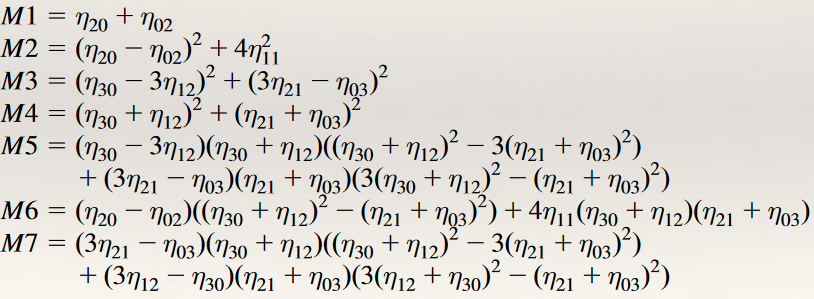
\includegraphics[scale=0.4]{hu_moments}\\
	\\
	There's another common set of rotation invariant moments called \textit{Zernike moment} that are used a lot in medical imaging for describing the shape of tumours. There are other sets moments that can be even more invariant to shape transformation like \textit{Affine invariant moments} which are even invariant to skew.
	\subsection{Boundary Description}
	\textbf{Chain Codes} are a simple way of encoding a boundary. You walk around the boundary and encode the direction you take on each step as a number, then cyclically shift the code so it forms the smallest possible integer value making it invariant to the starting point.\\
	In simple terms, you encode movement along the boundary to create a code.\\
	This can be made rotation invariant if you encode the \textit{differences} in direction rather than absolute values.\\
	It can also be made scale invariant if you resample the component to a fixed size but this doesn't work well in practice.\\
	Chain Code can be used for computing perimeter area, moments, etc... The perimeter for an 8-connected chain code is N(even numbers) + $\sqrt{2}$N(odd numbers). Practically speaking this is not so good for shape matching because there are problems with noise, resampling effects and it is difficult to find good similarity/distance measures.\\
	The Fourier transform can be used to encode shape information by decomposing the boundary into a small set of frequency components. There are two main steps to consider, defining a representation of a curve (the boundary) and expanding the representation using Fourier theory. By choosing these steps carefully it is possible to create rotation, translation and scale invariant boundary descriptions that can be used for recognition etc...
	\subsection{Describing Multiple Shapes}
	In \textbf{Region Adjacency Graphs} you build a graph from a set of connected components where each node corresponds to a component and the nodes are connected if they share a border. You can then easily detect patterns in the graph and is invariant to non-linear distortions but NOT  to \textit{occlusion}.
	\subsection{Point Distribution Models}
	\textbf{Procrustes Analysis} is where you need to align all training points. All point-sets must have the same size and be about the origin, the generalised procrustes analysis is an iterative technique for achieving this:
	\begin{enumerate}
		\item Arbitrarily choose a reference shape, typically by selecting it among the available instances and centring it about the origin
		\item Superimpose all instances to current reference shape by computing the optimal translation, scaling and rotation for each
		\item Computer the mean shape of the current set of superimposed shapes
		\item If the Procustes distance\footnote{The Euclidean distance between [x1,y1,x2,y1,...] and [x'1,y'1,x'2,y'2,...]} between the mean and reference shape is above a threshold, set the reference to the mean shape and continue to step 2
	\end{enumerate}
	You can then form the data points into a shape matrix where each pair of columns contains the x,y coordinates of aligned corresponding points across the images, and each row corresponds to an image.\\
	You can apply PCA to learn a low-dimensional basis, $S^TS=Q\land Q^T$ and Q can be used to generate shapes from a low-dimensional weight vector $\omega$: $\upsilon=\omega Q^T$.\\
	\\
	Active Shape Models and Constrained Local Models extend a Point Distribution Model by also learning local appearance around each point. This is typically just as an image template.\\
	Using a constrained optimisation algorithm, the shape can be optimally fitted to an image with constraints of \textit{plausible shape} and \textit{good template matching}.\\
	\subsection{Active Appearance Models}
	AAMs go even further and model the global appearance of the shape using Eigenfaces. The optimiser fits the model to new images by searching for both plausible shaped and plausible global appearance.
	\subsection{Summary}
	There are many different ways to describe the shape of connected components but the choice really depends on the required invariance. Multiple shapes can efficiently be represented by a RAG which is very robust.\\
	Point distribution models apply PCA to x-y coordinate pairs across multiple images to produce a low-dimensional parametric model. ASMs/CLMs also model local appearance, and can use this to optimise the fit of the model parameters to match an image.
	
	\section{Local Interest Points}
	Finding stable\footnote{repeatable} interest points is a key problem in modern computer vision. Applications in areas such as tracking, matching, image alignment, making robust features for classification and search, robot navigation, 3D reconstruction, etc...\\
	A good interest point has invariance to brightness change both local and global, has sufficient texture variation in the local neighbourhood but not too much, and has invariance to changes between the angle/position of the scene to the camera.
	\subsection{How to find them}
	There are lots of types of interest point types to choose from so we focus on corner detection and blob detection.
	\subsection{Harris and Stephens Corner Detector}
	The basic idea is that you search for corners by looking through a small window and for if by shifting the window by a small amount in any direction gives a large change in \textbf{intensity}.\\
	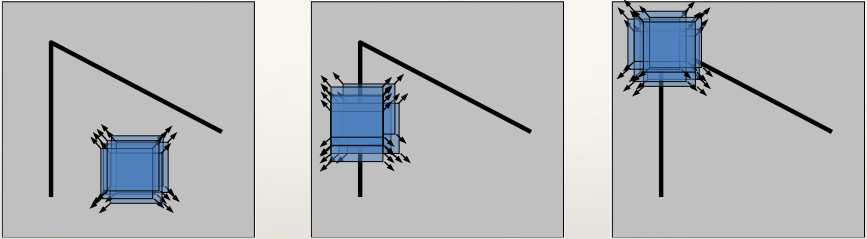
\includegraphics[width=\linewidth]{corner_shift}
	For a flat region there will be no change in all directions.\\
	For an edge there will be no change along the edge direction.\\
	But for a corner there will be change in all directions.\\
	The mathematical equation for this is as follows:
	$$E(x,y)=\sum_Wf(x_i,y_i)[I(w_i,y_i)-I(x_i+\Delta x,y_i+\Delta y)]^2$$
	The Taylor expansion allows ut to approximate the shifted intensity so by taking the first order terms we get this:\\
	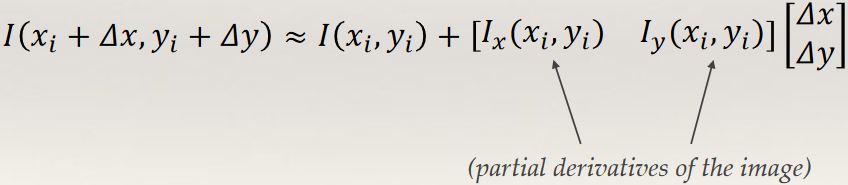
\includegraphics[width=\linewidth]{harris_math}
	By substituting and simplifying we get:
	$$[\Delta x \quad \Delta y]M[_{\Delta y}^{\Delta x}]$$
	\subsection{Structure Tensor}
	The square symmetric matrix M is called the \textbf{Structure Tensor} or the \textbf{Second Moment matrix}.\\
	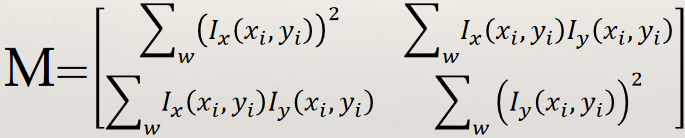
\includegraphics[width=\linewidth]{structure_tensor}
	It concisely encodes how the local shape intensity function of the window changes will small shifts. As with the 2D covariance matrix, the structure tensor describes an ellipse: $x^TMx=c$ which is in quadratic form. The eigenvalues and vectors tell us the rates of changes and their respective directions.
	SO MANY EQUATIONS AND i DONT KNOW WHAT THEY DO
	Rather than compute the eigenvalues directly, Harris and Stephens defined a corner response function in terms of the determinant and trace of M:
	$$det(M) = m_{00}M_{11}-M_{01}M_{10}=M_{00}M_{11}-M_{1-}^2 = \lambda_1\lambda_2$$
	$$trace(M) = M_{00}+M_{11}=\lambda_1+\lambda_2$$
	$$R=det(M)=k*trace(M)^2$$
	k is a small empirically set constant (usually 0.04 - 0.06)
	\subsection{Harris and Stephens Detector}
	It uses a simple algorithm where it takes all points with the response value above a threshold. Then keep only the points that are local maxima, so where the current response is bigger than the 8 neighbouring pixels.
	\subsection{Scale in Computer Vision}
	The problem with scale is that as an object moves closer to the camera it gets larger with more detail, and as it moves further away it gets smaller and loses detail. If you're using a technique that uses a fixed size processing window (e.g. Harris corners or anything using a fixed kernel) then this is a bit of a problem.\\
	\textbf{Scale space theory} is a formal framework for handling the scale problem. It represents the image by a series of increasingly smoothed/blurred images parametrised by a scale parameter t which represent the amount of smoothing. The key notion is that image structures smaller than sqrt(t) have been smoothed away at scale t.\\
	\\
	Many possible types of scale space are possible depending on the smoothing function but only the Gaussian function has the desired properties for image representation. These provable properties are called the \textit{"scale space axioms"}. Formally it is defined as $L(\cdot,\cdot;t)=g(\cdot,\cdot;t)*f(\cdot,\cdot)$\footnote{Convolution is over x,y for fixed t} where $t\geq0$ and
	$$g(x,y;t)=\frac{1}{2\pi t}e^{i(x^2+y^2)/2t}$$\footnote{$t=\sigma^2$=variance of the Gaussian}
	\\
	The \textbf{Nyquist-Shannon Sampling theorem} is as follows:\\
	\textit{If a function x(t) contains no frequencies higher than B hertz, it is completely determined by giving its ordinates at a series of points spaced 1/(2B) seconds apart.}\\
	So if you filter the signal with a low-pass filter that halves the frequency content, you can also half the sampling rate without loss of information.\\
	For the \textbf{Gaussian Pyramid} every time you double t in scale space, you can half the image size without loss of information. This leads to a much more efficient representation with faster processing and less memory.\\
	Extending the Harris and Stephens detector to work across scales is easy, we define a Gaussian scale space with a fixed set of scales and compute the corner response function at every pixel of each scale and keep only those with a response above a certain threshold.
	\subsection{Blob Detection}
	Recall that the Laplacian of Gaussian is a second derivative of a Gaussian used in the Marr-Hildreth edge detector with zero crossings of LoG convolution.\\
	By finding local minima or maxima you get a blob detector.\\
	The normalised scale space LoG defined as: $\bigtriangledown^2_{norm}L(x,y;t)=t(L_{xx}+L_{yy})$. By finding extrema of this function in scale space you can find blobs at their representative scale\footnote{about $~\sqrt{2t}$} you just need to look at the neighbouring pixels.\\
	A \textbf{very useful property} is that if a blob is detected at $(x_0,y_0;t_0)$ in an image, then under a scaling of that image by a factor s, the same blob would be detected at $(sx_0,sy_0;s^2t_0)$ in the scaled image.\\
	\\
	In practice it's computationally expensive to build a LoG scale space but the following approximation can be made:
	$$\bigtriangledown^2_{norm}L(x,y;t)\approx\frac{t}{\Delta t}(L(x,y;t+\Delta t)-L(x,y;t-\Delta t)$$
	This is called the \textbf{Difference of Gaussians}\footnote{DoG}, it implies that the LoG scale space can be built from subtracting adjacent scales of a Gaussian scale space.\\
	Of course, for efficiency you can also build a DoG pyramid. It is an \textit{oversampled} pyramid as there are multiple images between a doubling of scale. These images between a doubling of scale are an \textit{octave}.
	\subsection{Summary}
	Interest points have loads of applications in computer vision, they are robustly detected, and invariant to rotation, lighting change etc.\\
	We looked at two types, corners and blobs. \textit{Harris \& Stephens} is a common corner detector. Finding extrema in a multi scale DoG pyramid provides a robust blob detector.\\
	Scale space theory allows us to find features (corners and blobs) of different sizes.
	
	\section{Local Features and Matching}
	For local features multiple features are extracted, one per local interest point. The interest points are detected in the image and a feature is extracted from the surrounding pixels.\\
	These feature points are used for:
	\begin{itemize}
		\item Image Alignment
		\item Camera pose estimation and camera calibration
		\item 3D reconstruction
		\item Motion tracking
		\item Object recognition
		\item Indexing and database retrieval
		\item Robot navigation
	\end{itemize}
	For example when building a panorama we need to match and align the images. To do this we detect feature points in both images, find corresponding pairs and use the pairs to align the images.\\
	The first problem is being able to detect the same points independently in both images so we need a repeatable detector.\\
	The second problem is that for each point we need to correctly identify the corresponding point so we need an invariant, robust and distinctive descriptor.\\
	In stereo vision\footnote{3D} there are two important concepts related to matching:
	\begin{itemize}
		\item Narrow Baseline Stereo
		\subitem When the images are very similar
		\subitem This means the image capture points were close together
		\subitem Applicable for tracking where the object doesn't much a lot between frames
		\item Wide Baseline Stereo
		\subitem When the images are different
		\subitem This means the image capture points were far apart
		\subitem Applicable for generic matching tasks such as object recognition
	\end{itemize}
	\subsection{Robust Local Description}
	The descriptor requirements depend on the task. For a narrow baseline it doesn't need robustness to rotation and lighting and the descriptiveness can be reduced as the search is over a smaller area. For a wide baseline it needs to be robust to intensity change and invariant to rotation, it also needs to be highly descriptive to avoid mismatches\footnote{but not too distinctive it cannot find matches}, it must also be robust to small localisation errors of the interest point so the descriptor should not change too much if we move by a few pixels but would change more rapidly once we move further away.
	\subsection{Template Matching}
	A.k.a Matching by Correlation.\\
	For a narrow baseline you use local search windows based on the interest point in the first image. The template can then be matched against target interest points in the second image.\\
	The problems with wider baseline is that it isn't robust to rotation, it's sensitive to localisation of the interest point which is a problem for larger search windows, and with wider baselines you can't assume a search area because you need to consider all the interest points in the second image which makes it more likely to mismatch.
	\subsection{Local Intensity Histograms}
	You can describe the area around each interest point with a pixel histogram and then match each interest point in the first image to the most similar in the second image by measuring the Euclidean distance between the histograms.\\
	The problem is they are not necessarily very distinctive as many interest points will likely have similar histograms. They are also not rotation invariant if the sampling window is square or rectangular but this can be overcome with a circular window. They are also not invariant to illumination changes are is sensitive to interest point localisation but this can be solved.\\
	You want to allow the interest point to move a few pixels in any direction without changing the descriptor, apply a weighting so that pixels near the edge of the sampling patch have less effect and those nearer the interest point have more. It is common to use a Gaussian weighting centred on the interest point.\\
	Illumination invariance can be overcome by normalising or equalising the pixel patches before constructing the histogram or by using:
	\subsection{Local Gradient Histograms}
	From the partial derivatives of an image, that can be gathered from applying convolution with Sobel, it is easy to compute the \textbf{gradient directions and magnitudes}.
	$$\theta=atan2(\frac{\delta }{\delta y},\frac{\delta f}{\delta x})\quad m=\sqrt{(\frac{\delta f}{\delta x})^2+(\frac{\delta f}{\delta y})^2}$$
	Instead of building histograms of the raw pixel values we could instead build histograms that encode the gradient magnitude and direction for each pixel in the sampling patch. These are \textbf{invariant to brightness} change and are more distinctive.\\
	To build the histograms you quantise the directions in degrees into bins, usually around 8. Then for each pixel in the sampling patch you accumulate the gradient magnitude of that pixel in the respective orientation bin.\\
	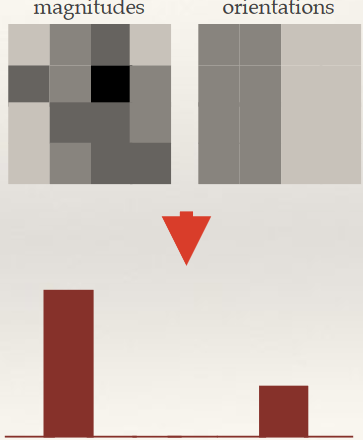
\includegraphics[width=0.4\linewidth]{gradient_histogram}\\
	Naturally these are not rotation invariant but can be made that way by finding the dominant orientation and shifting the histogram so that the dominant orientation is in the first bin.\\
	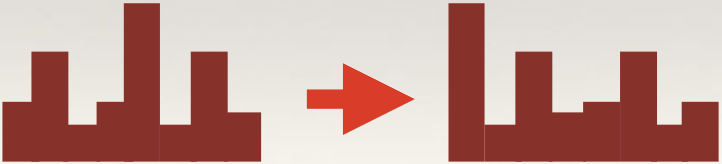
\includegraphics[width=\linewidth]{histogram_rotation}
	\subsection{The SIFT Feature}
	The \textbf{SIFT}\footnote{Scale Invariant Feature Transform} feature is widely used. It builds on the idea of a local gradient histogram bu incorporating \textit{spatial binning}, which in essence creates multiple gradient histograms about the interest point and appends them all together into a longer feature. Standard SIFT geometry appends a spatial 4x4 grid of histograms with 8 orientation leading to a 128 dimensional feature which is both highly discriminative and robust!\\
	You take the interest point and build a sampling patch either with a fixed size or a proportion to the scale of the interest point. You then apply a Gaussian weighting with lower weighting near the edges effectively making the corners have zero weight producing a circular sample region.\\
	By creating spatial bins you can split the area into 4x4 bins and create a gradient histogram for each using the previous Gaussian weighting. The orientations are measure relative to the overall dominant orientation of the patch.
	\subsection{Matching SIFT Features}
	The simplest way to match SIFT features is to take each feature in turn from the first image and find the most similar in the second image. Thresholding can be used to reject poor matches but unfortunately it doesn't work well and results in a lot of mismatches. \\
	A better solution is to take each feature from the first image, and find the two closest features in the second image. You only form a match if the ratio of distances between the closest and second closest matches is less than a threshold. This is typically set to 0.8 meaning that the distance to the closest feature must be at most 80\% of the second closest.\\
	This leads to a much more robust matching strategy.
	\subsection{Summary}
	Features extracted around interest points have lots of practical uses in computer vision.\\
	Matching scenarios basically fall into two categories. \textbf{Narrow-baseline} where the difference in images is slight, local image templates are often suitable descriptors. \textbf{Wide-baseline} where there are bigger differences in pose, gradient histogram descriptors are good here, especially \textbf{SIFT}.
	
	\section{Consistent Matching}
	When it comes to finding matching interest points across images we need a way to eliminate mismatches. Even the most advanced local feature can be prone to being mismatched because there is always a trade-off in feature distinctiveness. If it's too distinctive it won't match with subtle variation due to noise but if it's not distinctive enough it will match everything.\\
	We can use \textbf{Constrained matching} where we assume we are given a number of correspondences between the interest points in a pair of images. Would it then be possible to estimate which of the correspondences are \textbf{inliers}\footnote{correct} or \textbf{outliers}\footnote{incorrect} and what assumptions would we need to make?\\
	By assuming a geometric mapping between the two scenes can we recover that mapping and eliminate the mismatches?
	\subsection{Geometric Mapping}
	There are different types of \textbf{geometric transforms}:
	\begin{itemize}
		\item Point Transform
		\subitem $x'=Tx$
		\subitem T is the transform matrix
		\item Affine Transform
		\subitem $x'=Ax+b$
		\subitem 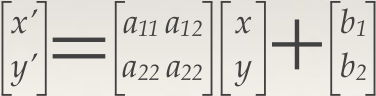
\includegraphics[width=0.2\linewidth]{affine_A}
		\subitem It is convenient to simplify this to
		\subitem 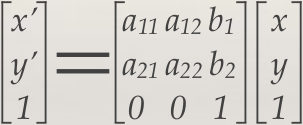
\includegraphics[width=0.2\linewidth]{affine_B}
		\item Translation
		\subitem 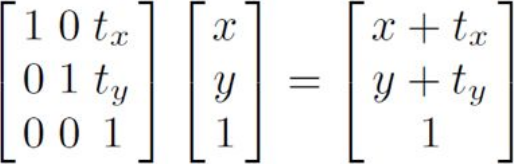
\includegraphics[width=0.3\linewidth]{translation}
		\item Translation and Rotation
		\subitem 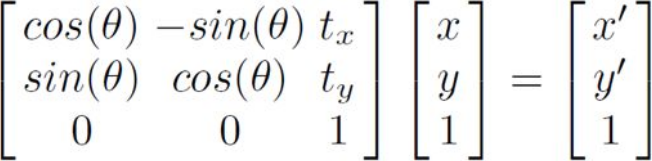
\includegraphics[width=0.3\linewidth]{rotation}
		\item Scaling
		\subitem 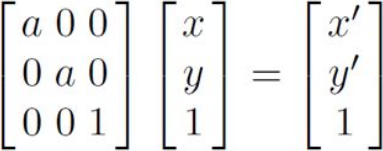
\includegraphics[width=0.2\linewidth]{scale}
		\item Aspect Ration
		\subitem 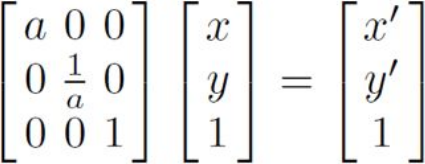
\includegraphics[width=0.2\linewidth]{aspect}
		\item Shear
		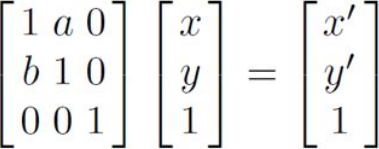
\includegraphics[width=0.2\linewidth]{shear}
	\end{itemize}
	So the \textbf{Affine Transform }has 6 DoF: translation, rotation, scale, aspect ration and shear!\\
	A \textbf{Similarity Transform}, however, only has 4 DoF: translation, rotation and scale.\\
	We can add an additional degree of freedom by normalising with $w$ so that the transformed vector is $[\cdot,\cdot,1]$, $x'=u/w\quad y'=v/w$.\\
	There's some slide that says \textbf{Homogeneous coordinates} whatever that means and it has a 1x3 vertical matrix that goes wx' then wy' then w. It's in lecture slides 8 just take a look.
	\subsection{Recovering a Geometric Mapping}
	It is possible to estimate a transform matrix from a set of point matches by solving a set of simultaneous equations. You need at least 4 point matches to solve a Homography or 3 to solve an affine transform.\\
	We don't need to know the solution but rather that in the presence of noise, and with potentially more matches than required, that we have to solve an \textit{overdetermined system}. We need to seek the minimum error or \textbf{least-squares} solution.
	\subsection{Least-Squares}
	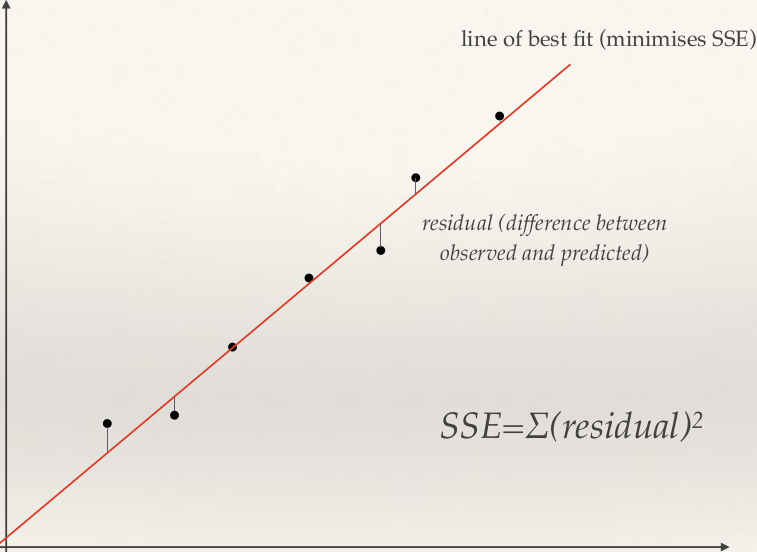
\includegraphics[width=\linewidth]{least_squares}
	I'm jsut going to have to look through these slides I don't understand what's going on without explanation.
	\subsection{Robust Estimation}
	The problem is noisy data, we need a way to deal with estimating a model in the presence of high amounts of noise\footnote{mis-matches}.\\
	Least-squares will be highly suboptimal and will probably find a very bad solution. Ideally we want to identify correct data and the bad data, then estimate the model using only the good data.\\
	The problem of learning a model in the presence of inliers and outliers comes under an area of mathematics called \textbf{robust estimation} or \textbf{robust model fitting}. There are a number of techniques but we'll see one of the simplest.
	\subsection{RANSAC}
	\textbf{RAndom SAmple Consensus}\\
	Assume that M data items required to estimate model T and that there are N data items in total.\\
	Algorithm:
	\begin{enumerate}
		\item Select M data items at random
		\item estimate model T
		\item find how many of the N data items fit T within tolerance \textit{tol}, call this K\footnote{basically compute how many times the absolute residual is less than tol}. The points that have an absolute residual less than \textit{tol} are the inliers; the other points are outliers.
		\item if K is large enough, either accept T, or compute least-squares estimate using all inliers, and exit with success.
		\item repeat 1..4 n iterations
		\item fail - no good T fit of data
	\end{enumerate}
	\subsection{Further Applications of Robust Local Matching}
	\textbf{Object Recognition}, the image of the object is matched against the scene, and recognised if there is a consistent match.\\
	\textbf{Augmented Reality}, the data can be added to a scene on the basis of the match.\\
	It's possible to estimate depth, and ultimately build a complete 3D scene from sets of point correspondences formed from matching local features.\\
	\\
	Image features can also be used to match music! This is how Shazam works, a recording of a piece of music can be turned into a picture called a spectrogram. Local image features can be extracted, described and matched from the spectrogram images.
	\subsection{Problems with Direct Local Feature Matching}
	A typical 800x600 image might have about 2000 DoG interest points/SIFT descriptors. Each SIFT descriptor is 128 dimensions, now assume you want to match a query image against a database of images, the distance between every query feature and every other feature needs to be calculated. Can this be optimised?
	\subsection{K-D Trees}
	These have a binary tree structure that partitions the space along axis-aligned hyperplanes, typically take each dimension in turn and splits on the median of the points in the enclosing partition. It then stops after a certain depth, or when the number of points in a leaf is less than a threshold.\\
	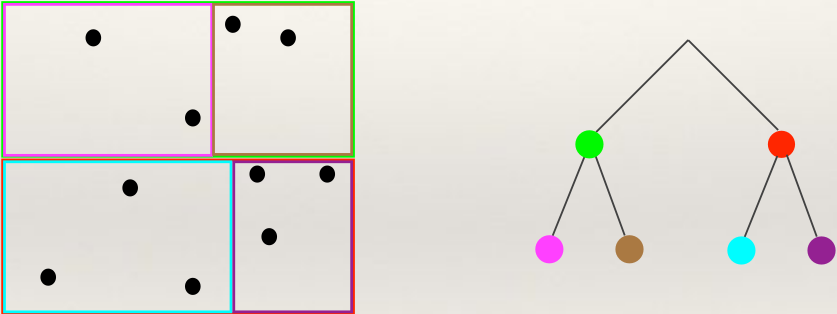
\includegraphics[width=\linewidth]{kd}
	You search by walking down the tree until a leaf is hit, and then brute-force search to find the best leaf. This isn't guaranteed to be the best though, you have to walk back up the tree and only stop once a root is reached\footnote{You do not have to check a subtree if it's clear it's further than the current best}.\\
	The problems are that it doesn't scale well to high dimensions as you tend to need to search most of the tree, and these are \textit{approximate} versions that won't necessarily return the exact answer that does scale if you don't mind the potential for mismatch.
	\subsection{Hashing}
	LSH (Local Sensitive Hashing) creates hash codes for vectors such that similar vectors have similar codes.
	\subsection{Sketching}
	A technique called sketching concatenates binary hashes into a bit string, with the correct LSH function, the Hamming distance between a pair of sketches is proportional to the Euclidean distance between the original vectors.\\
	You can easily compress SIFT features to 128 bits, the Hamming distance computation is cheap because it uses lookup tables and bitwise operations.
	\subsection{Summary}
	Inconsistent local feature matches can be removed assuming some form of constraint holds between the two images, this is usually a geometric mapping using affine transform or homography. It can be estimates by finding the least-squares solution of a set of simultaneous equations.\\
	Robust methods such as RANSAC allow inliers and outliers to be determined whilst learning the mapping.\\
	Interest point mapping is slow but K-D trees and Hashing can help.
\end{document}